\documentclass{article}
\usepackage[utf8]{inputenc}
\usepackage[greek,english]{babel}
\usepackage{alphabeta}
\usepackage{fancyhdr}
\usepackage{listings}
\usepackage{mathtools}
\usepackage{xcolor}
\usepackage{biblatex}
\usepackage[left=2cm,right=2cm]{geometry}

\lstset {
        basicstyle=\ttfamily,
        columns=fullflexible,
        breaklines=true,
        keepspaces=true
}

\title{Εργαστήριο Παράλληλου Υπολογισμού - Εργασία 1}
\author{Χρήστος Μαργιώλης}
\date{Νοέμβριος 2020}

\begin{document}

\begin{titlepage}
    \maketitle
\end{titlepage}

\renewcommand{\contentsname}{Περιεχόμενα}
\tableofcontents

\section{Τεκμηρίωση}
Το πρόγραμμα εν ολίγοις έχει την εξής επαναληπτική δομή:
\begin{itemize}
        \item Διαβάζονται στον επεξεργαστή 0 τα δεδομένα από τον χρήστη
        \item Διαμοιράζει στους υπόλοιπους επεξεργαστές τα δεδομένα που δώθηκαν
        \item Γίνονται οι κατάλληλες συγκρίσεις και έλεγχοι
        \item Ο επεξεργαστής 0 συλλέγει όλα τα αποτελέσματα και εμφανίζει
                αν ο πίνακας εν τέλει είναι ταξινομημένος ή όχι, και αν όχι, σε
                ποιο στοιχείο χάλασε η ταξινόμηση
        \item Εμφανίζει ένα μενού επιλογών ώστε να συνεχίσει ή να τερματιστεί το
                πρόγραμμα
\end{itemize}

Είναι σημαντικό να εξηγηθεί το πώς ισοκατανέμεται ο υπολογιστικός φόρτος σε όλους
τους $p$ επεξεργατές. Αφού διαβαστεί το $N$, δηλαδή το πόσα στοιχεία
έχει η ακολουθία $T$, το διαιρούμε δια όσους επεργαστές έχουμε. Αρχικά, ας
υποθέσουμε ότι το $N$ ειναι ακέραιο πολλαπλάσιο του $p$, και ότι
έχουμε - αν το $N$ για παράδειγμα είναι 10 και οι επεξεργαστές 2, τότε
$N / p = 10 / 2 = 5$ στοιχεία από τον συνολικό πίνακα για κάθε επεξεργαστή.

Πρέπει όμως να καλύψουμε και την περίπτωση που το $N$ δεν είναι ακέραιο πολλαπλάσιο του
$p$, για παράδειγμα $N = 7$ και $p = 2$. Στην περίπτωση αυτή θα πάρουμε το αποτέλεσμα
της πράξης $N \mod p$ η οποία θα μάς δώσει τον αριθμό των περισσευούμενων στοιχείων που
πρέπει να κατανεμηθούν.

Όταν ξεκινάει το loop για την διαμοίραση του υπολογιστικού φόρτου, πρέπει κάθε φορά
να υπολογίζουμε το μέγεθος του buffer που θέλουμε να σταλεί στον εκάστοτε επεξεργαστή.
Έπειτα υπολογίζουμε το offset - δηλαδή από ποιά θέση του αρχικού πίνακα και μετά - θα 
στείλουμε, παίρνοντας πάντα υπόψη τα τυχόν περισσευούμενα στοιχεία (αν υπάρχουν). Αν τύχει
και υπάρχουν περισσευούμενα, κάποιοι επεργαστές θα παραπάνω στοιχεία μέχρι να έχει
καλυφθεί ο αριθμός τον περισσευούμενων στοιχείων. Πρέπει να τονιστεί ότι έχω φροντίσει
οι επεξεργατές να έχουν διαφορά εώς ενα στοιχείο όσο αφορά την διαμοίραση, δηλαδή
αν υποτοθεί ότι $N = 5$ και $p = 2$ πρέπει να αποφύγουμε για παράδειγμα το να έχει
ο $p_0$ 4 στοιχεία και ο $p_1$ 1 στοιχείο - θέλουμε ο $p_0$ να έχει 3 στοιχεία
και ο $p_1$ 2.

Αφού υπολογίσουμε το offset, βρίσκουμε ποιό είναι το τελευταίο στοιχείο του 
προηγούμενου επεξεργαστή ώστε να μπορούμε να το συγκρίνουμε με το πρώτο στοιχείο
του επόμενου. Για να γίνει κατανοητό το γιατί χρειάζομαστε αυτόν τον επιπλέον έλεγχο,
ας υποθέσουε ότι έχουμε την ακολουθία
\[1, 2, 6, 3, 4, 5, 1, 2, 4, 1, 2, 3\]

Για $p = 4$ αυτή η ακολουθία θα μοιραστεί ως εξής
\[p_0 = 1, 2, 6\]
\[p_1 = 3, 4, 5\]
\[p_2 = 1, 2, 4\]
\[p_3 = 1, 2, 3\]

Στην περίπτωση που δεν πάρουμε υπόψη το τελευταίο στοιχείο του προηγούμενου
επεξεργαστή, βλέπουμε ότι όλοι οι επεξεργαστές θα μάς επιστρέψουν πως οι υπο-ακολουθίες
τους είναι ταξινομημένες, ενώ στον γενικό πίνακα, προφανώς, δεν είναι. Όμως, με τον
τρόπο που προανέφερα, μπορούμε να είμαστε σίγουροι ότι ο κάθε επεξεργαστής έχει
εις γνώσην του τί υπάρχει πριν από αυτόν, και χρειάζεται να γνωρίζει μόνο το τελευταίο
στοιχείο του προηγούμενού του, εφόσον μονο στις θέσεις $p_n[end]$ με $p_{n+1}[0]$ μπορεί να
υπάρξει λάθος ταξινόμηση και να μην το κατάλαβει το πρόγραμμα.

Αφού ο επεξεργαστής 0 στείλει στους υπόλοιπους επεξεργαστές τα κατάλληλα δεδομένα,
θα ξεκινήσουν από όλους τους $p$ επεξεργαστές οι συγκρίσεις ώστε να δούμε
αν η κάθε ακολουθία ήτανε ταξινομημένη. Η μία περίπτωση στην οποία η ακολουθία δεν θα
είναι ταξινομημένη είναι να ισχύει η συνθήκη $T_i > T_{i+1}$. Η άλλη περίπτωση
είναι να ισχύει ότι $T_i < prev$, δηλαδή το τελευταίο στοιχείο του προηγούμενου
επεξεργαστή να είναι μεγαλύτερο από το τρέχον στοιχείο στην ακολουθία.
Σημείωση ότι αυτή η περίπτωση ελέγχεται μόνο στην περίπτωση που \textit{δεν} είμαστε
στον επεξεργαστή 0, εφόσον αυτός δεν έχει κάποιον προηγούμενο επεξεργαστή.

Τα αποτελέσματα συλλέγονται όλα στον επεξεργαστή 0, ο οποίος έχει μερικές επιπλέον
μεταβλητές που θα καθορίσουν τα τελικά αποτελέσματα. Η πιο σημαντική είναι η
\lstinline{f_sorted} - αυτή η μεταβλητή θα μάς πει στο τέλος αν ο γενικός πίνακας ήτανε
ταξινομημένoς. Για να υπολογιστεί κάτι τέτοιο, ενώνουμε με AND όλες τις \lstinline{sorted}
flags που προέκυψαν από τις συγκρίσεις προηγούμενως. Ο λόγος που επέλεξα την πράξη
AND είναι γιατί αν έστω και μία από τις \lstinline{sorted} έτυχε να είναι 0, τότε και
η \lstinline{f_sorted} θα γίνει 0, ασχέτως του αν όλες οι άλλες \lstinline{sorted} ήτανε
1 ή όχι.

Τέλος, αφού βρεθεί αν ο πίνακας είναι τελικά ταξινομημένoς ή όχι, ο επεξεργαστής 0
θα τυπώσει ένα κατάλληλο μήνυμα. Αν ο πίνακας δεν είναι ταξινομημένος, θα τυπώσει
και ποιο είναι το πρώτο στοχείο που χάλασε την ταξινόμηση. Έπειτα θα εμφανιστεί το
μενού επιλογών.

\section{Κώδικας}
\lstinputlisting[language=C]{ex1.c}

\section{Προβλήματα}
Επειδή έκανα την ανάπτυξη του κώδικα κατά βάση σε FreeBSD, αλλά έκανα και tests
σε Arch Linux, παρατήρησα ότι στα Linux υπάρχει πιθανότητα η \lstinline{printf()}
να μην βγάζει output, ή αν βγάζει, να μην εμφανίζεται με την σωστή σειρά, ή ακόμα
και να κρεμάει όλο το πρόγραμμα. Σε διάφορες αναζητήσεις είδα ότι αρκετοί πρότειναν
την συνάρτηση \lstinline{fflush(stdout)} αλλά δεν είχα ιδιαίτερη τύχη με αυτή.
Αυτό που δούλεψε ήτανε να βάλω \lstinline{getchar()} όπου έβλεπα ότι χρειαζόταν,
και να προσθέσω newlines σε όλες τις \lstinline{printf()} που κανονικά δεν είχανε.

Ένα άλλο πρόβλημα που αντιμετώπισα ήτανε ότι όταν πρωτοέφτιαξα το menu επιλογών, δεν
έστελνα στους υπόλοιπους επεξεργαστές την επιλογή που έδινα στον επεξεργαστή 0,
το οποίο σήμαινε ότι οι υπόλοιποι επεξεργατές δεν ήξεραν τί είχα όντως απαντήσει,
οπότε μπορεί να εκτελούσαν και αυτοί το μενού, και γενικώς υπήρχε περίεργη
συμπεριφορά. Το διόρθωσα αυτό βάζοντας ένα απλό \lstinline{MPI_Send()} και
\lstinline{MPI_Recv()} αφού δώσω την επιλογή στον επεξεργαστή 0, ωστέ όλοι οι
υπόλοιποι να γνωρίζουν ότι δώθηκε απάντηση, καθώς και ποια ήτανε αυτή.

Δεν κατάφερα να βρω έναν καλό τρόπο ώστε να μπορώ να υπολογίσω την θέση του
στοιχείου που χαλάει την ταξινόμηση στον γενικό πίνακα. Δηλαδή, για παράδειγμα
αν τύχαινε στον επεξεργαστή 2 να χαλάσει το στοιχείο 1, θα έπρεπε να υπολογίσω
γενικώς στον συνολικό πίνακα ποια θέση έχει αυτό το στοιχείο. Οπότε, αντ'αυτού
έβαλα να εμφανίζεται η τιμή του στοιχείου που χαλάει την ταξινόμηση, και όχι την
θέση του. Βέβαια, κάτι τέτοιο γνωρίζω ότι δεν έχει ιδιαίτερο νόημα.

\section{Ενδεικτικά τρεξίματα}
Τα παρακάτω τρεξίματα έγιναν σε Arch Linux, εξ'ού και τα newlines που ανέφερα
στα προβλήματα και χαλάνε την εμφάνιση του πρόγραμματος.

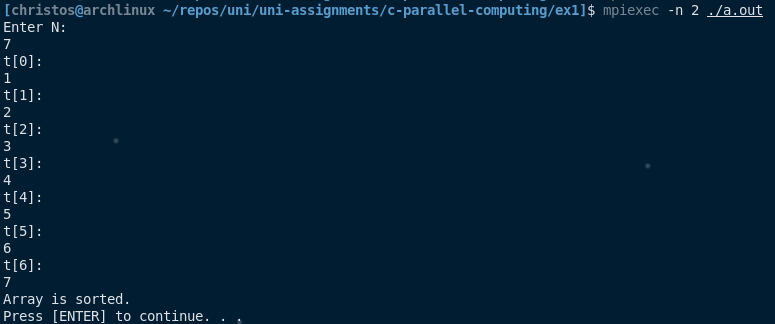
\includegraphics[width=\textwidth]{res/exmpl1.png}
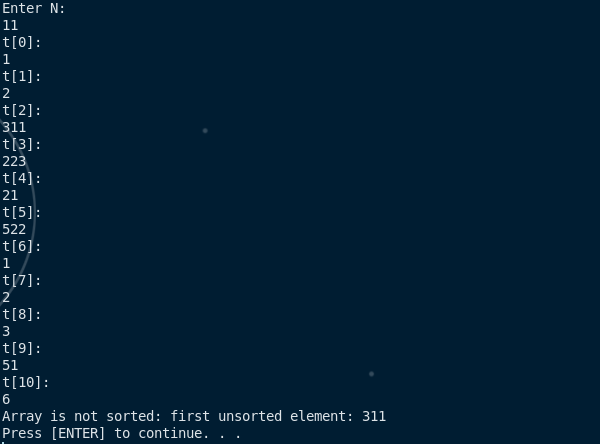
\includegraphics[width=\textwidth]{res/exmpl2.png}
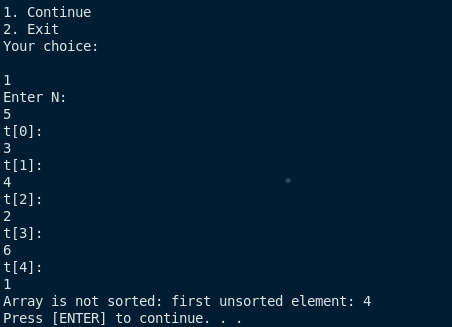
\includegraphics[width=\textwidth]{res/exmpl3.png}

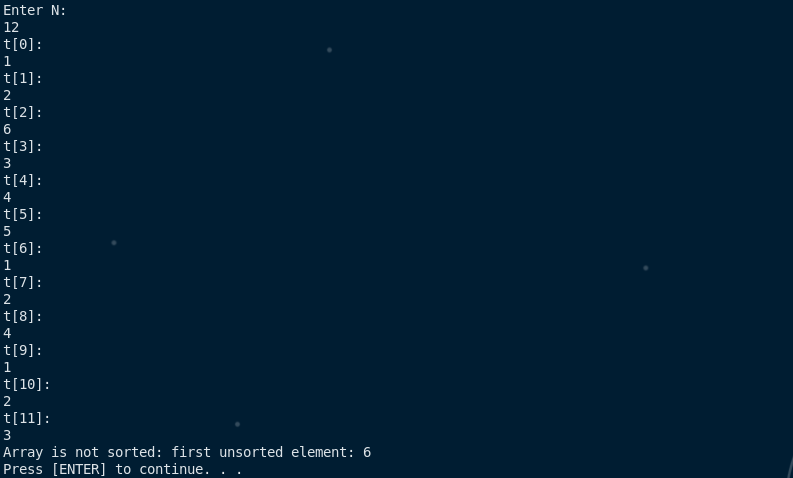
\includegraphics[width=\textwidth]{res/exmpl4.png}
Σε αυτό το τρέξιμο έδωσα την λίστα που έφερα ως παράδειγμα πιο πάνω
και ανέφερα ότι αν δεν ο κάθε επεξεργαστής δεν ξέρει ποιο είναι το προηγούμενο από
αυτόν στοιχείο, δεν μπορούμε να έχουμε σωστό αποτέλεσμα.

\end{document}
